\chapter{Introduction}
\label{ch:Introduction}
\index{Intro!Introduction}
\chaptertoc
\noindent

\section{Overview}
\label{sec:intro_overview}
\index{Intro!Overview}

% -------------------------------------------------------
% Keywords
% -------------------------------------------------------
% - process: a process is the instance of a computer program that is being executed by one or many threads.
% - processors/processor cores: central processing unit (CPU)—also called a central processor or main processor—is the most important processor in a given computer.
% - multi-core processor: is a computer processor integrated circuit with two or more separate processing cores, each of which executes program instructions in parallel.
% - parallelism: is difficult to define because it can appear on different levels.
% - parallel computing: parallel computing refers to the process of breaking down larger problems into smaller, independent, often similar parts that can be executed simultaneously by multiple processors communicating via shared memory.
% - types of parallel computing: bit-level parallelism, ilp, task parallelism.
% - parallel computer: is a machine which has more than one processors.
% - distributed memory machine: is a collection of single computers hooked up with network cables in that each processor can run an independent program and has its own memory without direct access to other processors' memory.
% - supercomputer: supercomputers play an important role in the field of computational science, and are used for a wide range of computationally intensive tasks in various fields. A supercomputer is a computer with a high level of performance as compared to a general-purpose computer. 
% - computer cluster: a computer cluster is a set of computers that work together so that they can be viewed as a single system.
% - HPC: High-performance computing (HPC) uses supercomputers and computer clusters to solve advanced computation problems. High-performance computing (HPC) as a term arose after the term "supercomputing".[3] HPC is sometimes used as a synonym for supercomputing; but, in other contexts, "supercomputer" is used to refer to a more powerful subset of "high-performance computers", and the term "supercomputing" becomes a subset of "high-performance computing".

% -------------------------------------------------------
% From HPC to the objects and instruments of the thesis
% -------------------------------------------------------
\noindent High performance computing (HPC) has gained an important role in solving complex problems and accelerating scientific research. HPC implies using supercomputers to perform computationally intensive operations \cite{sterling2018hpc}. Compared to a general-purpose computer, a supercomputer indicates a machine with high-performance level. The architecture of high-performance computers is designed towards parallel computing that can quickly process such large amounts of data and perform advanced computations.\\
%This is why the architecture refers to parallel computing.\\

% -------------------------------------------------------
% Parallel computing: taxonomy, mem-architectures
% -------------------------------------------------------
Parallel computing is a computational approach in which problems are split into smaller pieces and solved in parallel. Defining parallelism is difficult because it can appear at different levels, e.g., bit-level, instruction-level, data-level, and task-parallelism level \cite{victor2010introhpc}. Over the past two decades, these terms are frequently used to denote parallel computers, which are machines with more than one processor. A processor in computer science is called central processing unit (CPU) that performs operations on a data source. One way to characterize parallel computers is based on the hardware support level, such as multi-core processors \cite{blake2009multicoreprocs} where a processor may consist of multiple cores and each core is a processing element. Another way is Flynn’s characterization \cite{flynn1972comtaxonomy} based on data flow and control flow, which is known as the following four types:
\begin{itemize}
	\item SISD: Single Instruction Single Data
	\item SIMD: Single Instruction Multiple Data
	\item MISD: Multiple Instruction Single Data
	\item MIMD: Multiple Instruction Multiple Data
\end{itemize}
Alongside multiple processors working together, efficient access to memory is a critical consideration. For this reason, we can characterize parallel computers through different types of memory access. The main distinction is between shared memory and distributed memory \cite{jacob2008numavsuma}. Shared memory enables all processors to access the same memory pool, while in distributed memory, each processor has its own physical memory and address space.\\
% Shared memory, exemplified by Uniform Memory Access (UMA) architectures, enables all processors to access the same memory pool. In contrast, the concept of distributed memory, while not a precise synonym for NUMA, is often associated with architectures featuring Non-Uniform Memory Access (NUMA). NUMA introduces a unique dynamic where the access speed to memory can vary for a process depending on whether it is accessing its local memory or that of another processor. This non-uniformity in memory access times is a characteristic feature of NUMA architectures, setting them apart from the uniform memory access experienced in UMA systems.

% -------------------------------------------------------
% Computer clusters and distributed memory machines/systems and parallel apps
% -------------------------------------------------------
Building upon the concept of parallel computers, a supercomputer today refers to a parallel compute cluster, also considered as a common example for distributed memory machines/systems. We define a cluster as a set of parallel computers (called compute nodes) that work together and effectively function as a single system. For example, the SuperMUC-NG supercomputer at the Leibniz Supercomputing Centre (LRZ) of the Bavarian Academy of Sciences and Humanities \cite{lrz2020supermucng} has more than 6400 nodes with 311040 cores and 719 TB memory in total. All nodes are connected to each other via high-speed network, where each node has its private memory, the same hardware, and the same operating system. However, in certain configurations, there may be variations in hardware or operating systems for specific purposes. The scale of clusters may be small as a two-node system or large with many nodes as a supercomputer like SuperMUC-NG. Regardless of the scale, the interconnection among nodes has to be across a network \cite{liem1991mddistributed}. When multiple nodes exchange data, a message-passing technique is needed; and in most cases the open library standard, Message Passing Interface (MPI) \cite{gropp1996mpich}, is used. Commonly, there are different parallel programming models, e.g., shared memory programming models, distributed memory or message passing programming models, data parallel models, and hybrid models. However, it is important to note that almost all applications should be broken into discrete pieces or smaller tasks. Then, the tasks can be executed simultaneously. We consider such applications as task or task-based parallel applications \cite{thoman2018taxonomy}. On one side, executing tasks in parallel should gain speedup in completion time. On the other side, challenges during execution are communication overhead, synchronization, and load balancing.\\

% -------------------------------------------------------
% Thesis' problem and use case: load balancing & iterative apps
% -------------------------------------------------------
\begin{figure}[t]
	\centering
	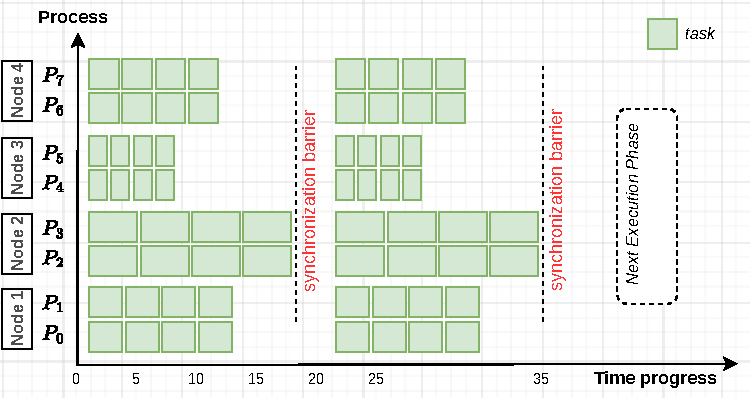
\includegraphics[scale=0.75]{./pictures/introduction/intro_usecase.pdf}
	\caption{An illustration of iterative execution and load imbalance in distributed memory systems with 4 compute nodes, 2 processes per node.}
	\label{fig:intro_usecase}
\end{figure}

This thesis is concerned with load balancing in distributed memory systems. The goal is to treat each processor with an equal share of the total load \cite{cybenko1989dynamic}. Load balancing is important because a load imbalance might affect the completion time of parallel applications. For example, we assume a given distribution, where each processor is assigned a number of tasks before execution. A processor executing tasks refers to a process that is defined as a logical instance at operating system level. During execution, when all processes are subject to a synchronization barrier but some of them are slower than others, the overall performance will be determined by load imbalance.\\

Regarding the definition of load, load in this thesis refers to the amount of time that a process executes tasks. Occasionally, we might use this amount of time, which a process is active to execute one or more tasks, as the execution time of tasks. Therefore, the values of load and execution time can be understood interchangeably. We target task-based parallel applications with iterative execution. A task is often defined by a compute function, where each task points to a code region and data. ``Iterative'' indicates applications with multiple execution phases that can be repeated over time steps based on user configuration. ``Iterative'' widely refers to bulk synchronous parallel (BSP) models \cite{valiant1990bridging}. Computation in BSP is divided into a sequence of execution phases as shown in Figure \ref{fig:intro_usecase}, which illustrates an iterative execution on 4 nodes, 2 processes per node. The x-axis is the time progress of task execution, where green boxes represent tasks and their length denotes the load value or the execution time. The y-axis lists compute nodes and processes executing tasks in each phase. A phase finishes when all processes are done. At the end of a phase, a barrier is used to ensure synchronization for the next phase.\\

% -------------------------------------------------------
% An overview about approaches in general
% -------------------------------------------------------
In consideration of dealing with imbalance at runtime, load balancing can be classified as ``static'' and ``dynamic'' \cite{xu1996load}.
\begin{itemize}
	\item ``Static'' means using the estimated execution time of tasks per process to balance the load before running applications. Thereby, an accurate cost model for either optimal task assignment or task partitioning algorithms is needed.
	\item ``Dynamic'' means scheduling tasks at runtime without prior knowledge about the load values. Application behavior and system performance variability might change these values at runtime.
\end{itemize}

Specifically, our work are concerned with dynamic load balancing approaches. There are two reference schemes of dynamic load balancing approaches: master-worker \cite{Riakiotakis2011MasterWorkerModel} \cite{Chronopoulos2005ScaleMasterWorkerModel} and work stealing \cite{Blumofe1999OriginWS} \cite{dinan2009scalable}.
\begin{itemize}
	\item Master-worker denotes a scheme, in which the master monitors and distributes the load to all workers. The downside of master-worker is that it is difficult to scale the number of compute nodes up because the master node can be overloaded by an increasing number of worker nodes. Instead of nodes, master process and worker process can be used as alternatives.
	\item Work stealing denotes that we allow an idle process to steal work\footnote{``\textit{Work}'' and ``\textit{task}'' might be used interchangeably.} from the busy ones without prior knowledge. Work stealing can be particularly effective, but its efficiency can be limited by communication overhead in distributed memory systems. Communication overhead can cause delays when processes exchange information and steal tasks.
\end{itemize}

In general, dynamic load balancing depends on a typical context. Our target is to balance the load of a given distribution of tasks over processes running on distributed memory systems. We explore various approaches through the lens of work stealing. The subsequent section outlines our research problem formulation and motivation.

% ``Overloaded'' indicates the load value of a process is larger than average. It also means the process is executing tasks slower than others.

%This drive to improve computation is accomplished by advancing the
%state-of-the-art of computer hardware and software.
%The notion of \gls*{HPC}, the advancement of what is computationally viable
%on computer systems, is also referred to as
%\gls{capability computing}~\cite[1]{NAC2008}.
%\index{HPC|textbf}\index{Capability computing}

% 1.2 Problem Definition and Motivation
% 1.1 Problem Statement
\section{Research Problem and Motivation}
\label{sec:intro_prob_form_motiv}
\index{Intro!Research Problem and Motivation}

\begin{figure}[t]
	\centering
	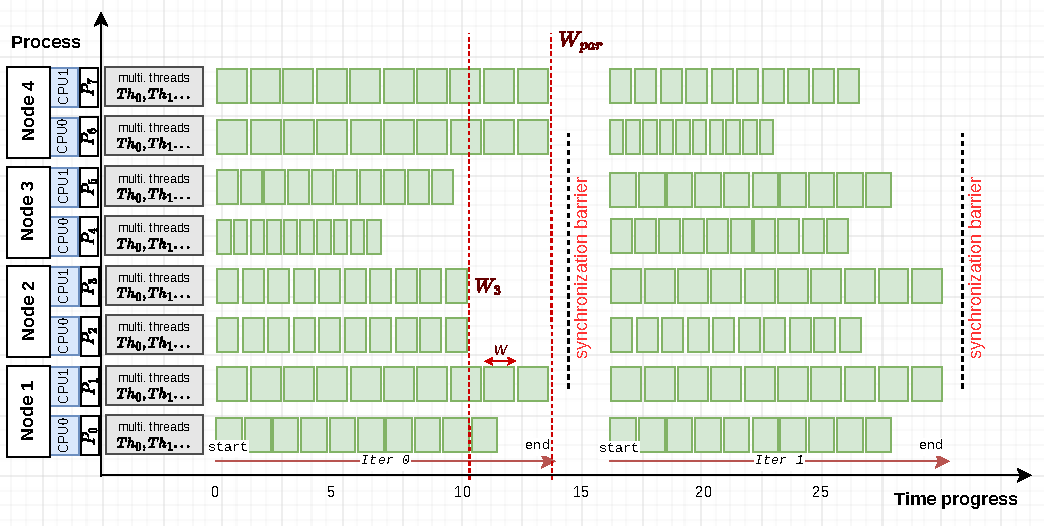
\includegraphics[scale=0.7]{./pictures/introduction/intro_problem_formulation.pdf}
	\caption{An illustration refers to a real iterative execution with load imbalance in task parallel application, running on 4 compute nodes, 2 processes per node, and multiple threads per process.}
	\label{fig:intro_prob_formulation}
\end{figure}

We illustrate the load imbalance context in Figure \ref{fig:intro_prob_formulation} to explain the problem formulation intuitively. This figure reveals a similar case shown in Figure \ref{fig:intro_usecase}, load imbalance at runtime on 4 compute nodes. Again with the x, y coordinates, the x-dimension shows the time progress, the y-dimension shows the involved processes within compute nodes but in more detail with the threads executing tasks on each process. We intend to highlight this illustration as a realistic execution and refer to a hybrid parallel programming model in practice, multiprocessing + multithreading. A modern processor today is mostly multicore architecture; hence, a process mapped to a processor can create multiple threads pinned to multiple corresponding cores within that processor.\\

Suppose we use MPI to leverage communication between processes, then the hybrid model is known as MPI+X \cite{rabenseifner2006mpiomp}. In Figure \ref{fig:intro_prob_formulation}, each process, e.g., $P_{0}$, $P_{1}$, indicates an MPI process (also called MPI rank). One MPI process can spawn multiple threads to execute tasks denoted by \texttt{multi.threads} ($Th_{0}$, $Th_{1}$, and so on). The term ``multiple threads'' refers to many threads, where a thread is the segment of a process. While processes are mostly isolated, threads share memory and data. Therefore, we assume tasks are automatically scheduled and fairly executed within a process. An imbalance at runtime comes from different processes across different compute nodes, not within a process. Before every execution phase, each process is assigned a given number of tasks, and this assignment normally follows the partitioning algorithm of an application called a given task distribution on processes. In Figure \ref{fig:intro_prob_formulation}, we highlight the first execution phase (denoted by Iteration 0 or \texttt{Iter 0} for short), where tasks belonging to process $P_{1}$, $P_{6}$, and $P_{7}$ are executed slower than the others, causing the load imbalance.\\

For comprehensive analysis, we formulate the problem as follows. Given $T$ tasks in total, the tasks are indexed from $\{0,...,(T-1)\}$ and distributed among $P$ processes before execution. When $T$ is mentioned as a set, we can understand it as $\{0,...,(T-1)\}$; when $T$ is mentioned as an integer number, it is the total number of tasks. Each process is denoted by $P_{i}$, where $i$ in the range of $\{0,...,(P-1)\}$. Similar to $T$, $P$ can be mentioned as the number of processes if it is an integer number or the set $\{0,...,(P-1)\}$. A scheduled task is atomic and runs on a specific thread until termination. Tasks, load values, and evaluation metrics are summarized in detail below.
\begin{itemize}
	\item $T_{i}$: a set of assigned tasks for process $P_{i}$, e.g., $T_{1}$ is the set of assigned tasks belonging to process $P_{1}$. When $T_{i}$ is mentioned as an integer number, it indicates the number of tasks assigned to process $P_{i}$.

	\item $w$: the load value of a task in general. The value of $w$ is also called a wallclock execution time and $w > 0$. When we refer to a load of a particular task in a set $T_{i}$ of process $P_{i}$, $w$ can be attached with an index $j$, which means task $j$ belongs to the set $T_{i}$. Overall, $T_{i}$ is a subset of $T$, and all tasks in $T_{i}$ belong to the set $T$. Therefore, a particular value $w_{j}$ must be $> 0$ and $j$ $\in$ $\{0,...,(T-1)\}$. The standard deviation between the values of $w$ determines the type of tasks, uniform or non-uniform. Uniform tasks indicate the tasks with approximate load values, while non-uniform tasks indicate the tasks with different load values resulting in a high standard deviation of the load values of tasks. In Figure \ref{fig:intro_prob_formulation}, the length of green boxes highlights the length of $w$. For this illustrated case, we can say that the load values of tasks in a process are uniform, but different tasks in different processes are non-uniform.
	
	\item $L_{i}, \forall i \in P$: the total load of process $P_{i}$, where $L_{i} = \sum_{j \in T_{i}} w_{j}$.
	
	\item $W_{i}, \forall i \in P$: the wallclock execution time of process $P_{i}$. Unlike $L_{i}$, $W_{i}$ indicates the completion time of process $P_{i}$ when all tasks are done. The execution of all tasks here indicates that they are executed in parallel by multiple threads in process $P_{i}$. Both $L_{i}$ and $W_{i}$ at the end will reflect the imbalance ratio. Figure \ref{fig:intro_prob_formulation} marks $W_{3}$ as an example to indicate $W_{i}$.
	
	\item $W_{par}$: the parallel wallclock execution time known as the completion time, makespan, or application time, $W_{par} = max_{i \in P}(W_{i})$. For example, in Figure \ref{fig:intro_prob_formulation} $W_{par}$ is determined by process $P_{6}$, $P_{7}$ at \texttt{Iter 0}.
	
	\item $R_{imb}$: imbalance ratio, $R_{imb} = \frac{W_{max}}{W_{avg}} - 1 = \frac{W_{par}}{W_{avg}} - 1$, where $W_{max}$ is the maximum wallclock execution time ($max_{i \in P}(W_{i}) = W_{par}$), and $W_{avg}$ is the average value ($avg_{i \in P}(W_{i})$). Alternatively, we can also calculate $R_{imb}$ via the total load values such as $R_{imb} = \frac{L_{max}}{L_{avg}} - 1$.
\end{itemize}

If $R_{imb} \approx 0$, there is no imbalance. If $R_{imb}$ is greater than or equal to a certain threshold, $R_{imb}$ is determined imbalance at runtime. For example, users define a threshold $0.2$, and $R_{imb} \geq 0.2$ is determined as an imbalance. In this case, $W_{par}$ is seen as unoptimized. Our work targets reducing the values of $R_{imb}$ and $W_{par}$.\\

In our context, task migration is the only way to perform dynamic load balancing because tasks are already distributed among compute nodes. At runtime, we cannot share or add more computing resources in distributed memory systems. Otherwise, the technology must be changed to enable sharing resources across separate machines.\\

As mentioned in Section \ref{sec:intro_overview}, the previous approaches are mostly based on two schemes of dynamic load balancing: master-worker and work stealing. When considered in principle, all of these approaches comprise four components to their operations \cite{xu1996load}. The four components can be explicit or implicit, including:
\begin{itemize}
	\item Load measurement: indicates monitoring, checking either the load status or the execution speed.
	\item Information exchange: indicates the operations of status exchange among processes. This operation helps to synchronize the execution status to calculate imbalance ratio.
	\item Initiation rule: implies when to initiate a balancing operation. It can be initialized by overloaded processes or underloaded processes or periodically at runtime.
	\item Load balancing operations: implies the actions used to balance the load, e.g., task migration, thread/process migration. There might be different rules \cite{xu1996load} for making decisions on these actions.

\end{itemize}

\begin{figure}[t]
	\centering
	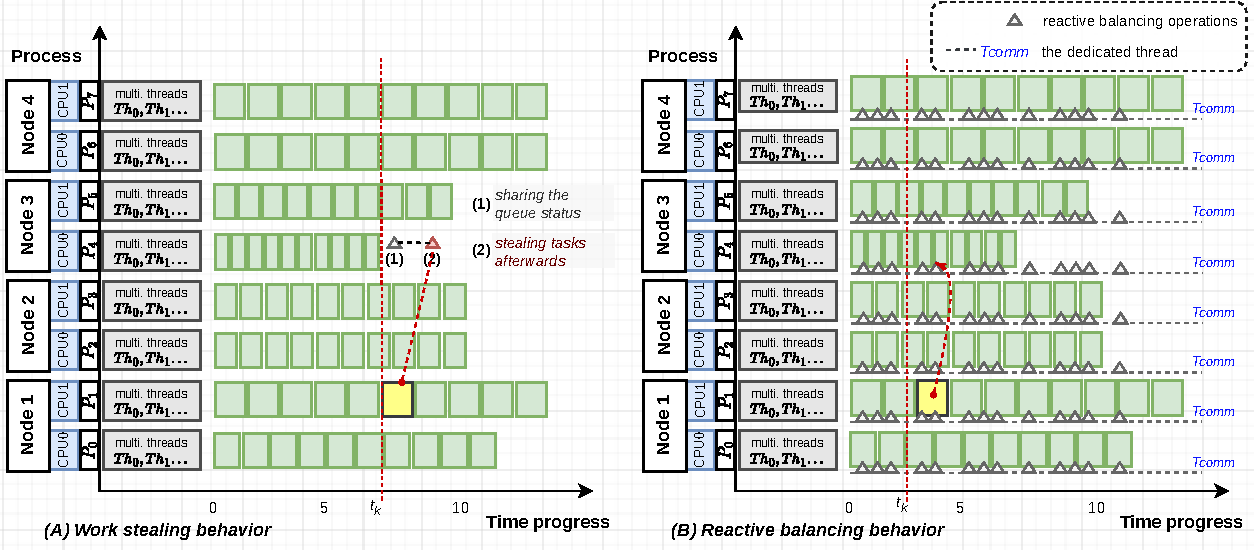
\includegraphics[scale=0.65]{./pictures/introduction/intro_motiv_workstealing_vs_reactlb.pdf}
	\caption{Behaviors of work stealing and reactive load balancing.}
	\label{fig:intro_motiv_workstealing_vs_reactlb}
\end{figure}

A master-worker scheme works as a centralized scheme, where the master is a central point, and workers wait to receive commands from the master. It is easy to manage load and control the balance of load, but it is challenging to scale up the number of distributed memory machines.\\

Work stealing is more relevant in our imbalance context. However, if we take communication overhead in distributed memory machines into account, the behavior of work stealing can be limited by the components of ``information exchange'' and ``load balancing operations''. The reasons are that tasks have to be migrated, and the behaviors of work stealing can make it too late to steal tasks. In a detailed inspection, these behaviors can refer to different variants. They are classified as follows.
\begin{itemize}
	\item Passive: indicates work stealing in distributed memory systems, which has several proposed approaches for HPC clusters \cite{ravichandran2011wsmulticorhpc} and also in-depth analysis of stealing-tasks behavior through performance modeling \cite{gast2021analysis}. The algorithms and behaviors of work stealing in distributed memory differ from shared memory because the global operations, such as synchronization primitives, caching, or coherence protocols, often result in high overhead and latency. Another point is a contention that may occur when multiple thieves try to steal tasks from the same victim process \cite{paudel2013meritdistws}. Therefore, in most algorithms for distributed memory, the decision of stealing tasks is taken when an idle process exists. Basically, the idle process sends out a steal request when its local queue is empty. Depending on a specific algorithm, the busy processes may also be in charge of responding to steal requests before a task is stolen. Thereby, we consider the behavior of processes performing work stealing in distributed memory systems as a passive action.\\
	
	 For illustration, Figure \ref{fig:intro_motiv_workstealing_vs_reactlb} (A) shows work stealing applied to the imbalance case illustrated in Figure \ref{fig:intro_prob_formulation}. The x-axis again represents time progress during execution, and the y-axis highlights the labels of compute nodes, processes with their executing-tasks threads. At time $t_{k}$, process $P_{4}$ is idle, then it needs to mainly perform: (1) sharing/exchanging the idle status with other processes, (2) stealing tasks afterward if one of the overloaded processes responds to the request. When an agreement is made, process $P_{4}$ steals a task from process $P_{1}$. The stolen task is denoted by the yellow box. As we can see, these behaviors can be too late if communication overhead is dominant, leading to missed requests, an unexpected number of stolen tasks, or even some overloaded processes that are not handled fairly.
	
%\noindent In work stealing, the bottleneck is obviously with migration overhead, and the time to make stealing decisions is too late. For reactive load balancing, we must assume that a shortcoming period is valid about the imbalance for reacting to task offloading. Even when we make reactive decisions, it might be challenging to decide how many tasks should be offloaded at once. Besides, choosing or pairing an offloader with a victim might be unfair and incorrect because of no prior knowledge about load at runtime, especially in high imbalance cases. Therefore, these points have motivated the thesis as follows:

	\item Active: indicates the behaviors as seen in the state-of-the-art approaches. Instead of waiting until a process is idle, we attempt to send tasks actively from one process to another beforehand, if the imbalance is speculatively observed or predicted. Depending on how much information we have in a specific context, we can divide ``active'' into two variants:
		\begin{itemize}
			\item Reactive: emphasizes responding to situations after certain conditions are satisfied. When an imbalance is detected periodically, this reacts with a decision of migrating or not migrating tasks. In particular, prior knowledge about load values is not needed. This reaction is only based on the most current status of execution and short-period speculation. After that, we perform these reactive operations repeatedly and continuously. Therefore, task migration here does not mean stealing tasks but offloading tasks\footnote{``Offload'' and ``migrate'' might be used interchangeably in this thesis} and we refer to reactive task offloading \cite{klinkenberg2020reactmig}.
			\item Proactive: emphasizes taking actions in advance based on anticipating/predicting the future. This means we know more details about the imbalance situation, e.g., how much imbalance and load value are. Therefore, proactive task offloading means offloading tasks earlier and more controllable than reactive task offloading.
		\end{itemize}
	
\end{itemize}

Several reactive load balancing approaches have been proposed \cite{Klinkenberg2020ChameleonReactLB} \cite{Samfass2021ChameleonReactRepLB}. These approaches continuously monitor the execution status instead of waiting for an empty queue. The monitored status information helps calculate imbalance ratio ($R_{imb}$) based on the queue length. Then, we can determine which process executes tasks slow and which process is fast. Following that, we can offload tasks from a slow process to a fast process reactively.\\

``Slow'' and ``fast'' imply overloaded and underloaded processes. For example, Figure \ref{fig:intro_motiv_workstealing_vs_reactlb} (B) shows a reference implementation with MPI+OpenMP \cite{rabenseifner2009hybrid}. One thread per process is dedicated to be a communication thread (called $Tcomm$). $Tcomm$ is used to overlap communication and computation. For reactive load balancing, $Tcomm$ on each process monitors the execution speed, shares this information with other processes, and calculates the imbalance ratio. These operations are continuous and repeated. If an imbalance is detected over a given condition, we can offload tasks promptly from a slow process to a fast one. For example, at time $t_{k}$ in Figure \ref{fig:intro_motiv_workstealing_vs_reactlb} (B), the imbalance is detected, and the reactive decision is made earlier than work stealing shown in Figure \ref{fig:intro_motiv_workstealing_vs_reactlb} (A). In this case, assuming that process $P_{1}$ is slow and process $P_{4}$ is fast as a good victim for offloading tasks. Victims in work stealing indicate the overloaded processes whose tasks are stolen. In reactive approaches, victims indicate the underloaded (fast) processes where tasks are offloaded to. The downside of reactive load balancing can be wrong speculation because we rely only on the most current status of execution speed. Periodically, reactive task offloading can be decided incorrectly under high imbalance cases. Besides, performance can be affected at the end when tasks are offloaded with an inappropriate number or wrong victims. \\

The limitations of work stealing and reactive load balancing motivate us to investigate a new proactive approach. In principle, our idea tries to tackle dynamic load balancing with the following constraints:
\begin{itemize}
	\item Performance slowdown at runtime causes imbalance, which is unknown before running applications. This refers to the inherent variation in supercomputer architectures with the design of today multicore CPUs. Acun et al. use compute-intensive kernels and applications to analyze the variation among processors in different supercomputers \cite{acun2016variturboboost}. They observe that there is an execution time difference of up to 16\% among processors under enabling Turbo Boost. The intrinsic differences in the chips’ power efficiency are the culprit behind the frequency variation. A similar work is from Weisbach et al. \cite{weisbach2018hwvariation}; they also show six orders of magnitude difference in relative variation among CPU cores across different compute platforms such as Intel x86, Cavium ARM64, Fujitsu SPARC64, IBM Power.
	\item Communication overhead is a bottleneck for exchanging execution status and migrating tasks. The communication overhead in distributed memory systems comes from:
		\begin{itemize}
			\item Latency ($\lambda$): time between sending and receiving the head of a message, where $\lambda$ does not depend on the size of a message.
			\item Delay time ($d$): time for transmitting an entire message between two nodes, where $d$ depends on the size of a message.
		\end{itemize}
	\item At runtime, we lack load information as well as system performance information to estimate better when, where, and how many tasks should be migrated at once.
\end{itemize}


% 1.3 Research Questions
\section{Research Questions}
\label{sec:intro_res_ques}
\index{Intro!Research Questions}

% in Section \ref{sec:intro_prob_form_motiv}
Based on the motivation above, this thesis focuses on the following two main research questions (RQs).
\begin{itemize}
	\item \textbf{RQ1: How can we model the behavior of reactive load balancing to understand its limits in distributed memory systems?}
	\item \textbf{RQ2: How can we proactively balance the load of task parallel applications at runtime?}
\end{itemize}

RQ1 indicates a performance model to analyze the limit of reactive load balancing as well as work stealing. Due to the overhead of balancing operations or task migration, they might reach a limit if actions are late and insufficient. The answer of RQ1 supports in-depth analysis and leads to a new approach mentioned in RQ2.\\

RQ2 introduces a novel proactive load balancing approach, where ``proactive'' means that task migration will be anticipated with prediction information. We use prediction information to estimate the number of tasks and potential victims for migrating tasks. Unlike work stealing or reactive load balancing, our approach is controlled proactively. Tasks can be migrated earlier when we have knowledge about load values.\\

To answer RQ2 comprehensively, we address two sub-questions (SQs):
\begin{itemize}
	\item SQ1: How can we predict the load of tasks at runtime to support proactive load balancing?
	\item SQ2: How can we proactively co-schedule tasks to balance the load?
\end{itemize}

In order to perform offloading tasks proactively, we need to know the load values of tasks and how much load is different between processes, indicating the difference between overloaded and underloaded values. SQ1 and SQ2 support each other to answer RQ2, detailing how proactive load balancing works. Typically, SQ1 asks for load prediction, which is necessary to calculate how much load is different. We can then determine which processes are potential and available for offloading tasks. SQ2 implies methods to guide task offloading, where ''co-schedule tasks`` implies not only how to migrate tasks among processes in an application to balance the load, but also migrate tasks across multiple applications to improve overall performance. The output of SQ1, predicted load values, is the input of SQ2. Importantly, the output of SQ2 comes to how many tasks should be migrated from which process to which process. In this thesis, ``approach'' implies a broader strategy and perspective that drives load balancing, while ``method'' refers to a structured procedure that is more specific and often includes steps to guide task offloading for load balancing.






% 1.4 Methodology and Contribution
\section{Methodology and Contributions}
\label{sec:intro_method_contribution}
\index{Intro!MethodologyContribution}

The methodology of this work is derived from experimental research. First, we conduct experiments on micro-benchmarks and real applications with different imbalance levels. Each experiment is deployed in distributed memory systems with and without load balancing at runtime. Second, we profile the execution to analyze the behavior of load balancing. Specifically, we deploy both work stealing and reactive load balancing. Upon thoroughly analyzing their runtime behaviors, we determine that overall performance is still limited, particularly in high imbalance cases. Notably, the decision taking actions in work stealing and reactive load balancing might be insufficient occasionally.\\

To explore a cause-and-effect relationship, we create a vector space of influence parameters. Then, we formulate the problem to support building a performance model for reactive load balancing. Drawing upon the performance model, a simulator is developed for further testing and proving the hypothesis. This methodology motivates us to investigate a new proactive load balancing approach.\\

Concretely, our work contributes a performance model to analyze the efficiency bound of reactive load balancing and work stealing. The model is represented as function $F$, where its inputs are the given information, including the distribution of $T$ tasks on $P$ processes, the load of tasks ($w$), and the constraints under communication such as latency, delay time when tasks are migrated. In $P$ processes, the inputs indicate the number of overloaded and underloaded processes. Following that, the proposed model can analyze performance in case of applying work stealing or reactive load balancing. With our performance model, we create a simulator to leverage the analysis by manipulating variables and collecting quantitative data. \\

Apart from the abstracted model, this work contributes a new proactive approach, in which ``proactive'' can improve dynamic load balancing further by anticipating the future and taking actions in advance. We can offload tasks earlier and thus more proactively. We propose this toward a proactive scheme for a task-based programming model. Our approach divides the main execution of parallel applications into two streams of execution: one is threads for executing tasks and another one is a dedicated thread for proactive load balancing. The dedicated thread is named $Tcomm$, which will manage (1) task characterization, (2) online load prediction, (3) proactive task offloading. (1) and (2) provide load information to better estimating the number of tasks and potential victims for offloading tasks. (3) can be performed with different task offloading methods based on the prediction knowledge. In particular, we show two methods and one extension of co-scheduling tasks:
\begin{itemize}
	\item Method 1: feedback task offloading
	\item Method 2: ML-based (Machine Learning-based) task offloading
\end{itemize}

The extension is co-scheduling tasks across multiple applications, which is considered as a new scheduling scheme in HPC clusters. For a long-term vision, we can co-schedule tasks from one application to another application during concurrent execution. Taking this into account, the benefit can be not only balancing load but also increasing compute resource utilization.



% 1.5 Publication
\section{Publications}
\label{sec:intro_publication}
\index{Intro!Publication}

The following publications are associated with the thesis. We split the publications into two groups linked directly or indirectly to the thesis. We refer to the contributor roles taxonomy named \textit{CRediT} at \url{https://casrai.org/credit/} to show the author's contribution to each paper.\\

There are some main roles used to describe the contribution:
\begin{itemize}
	\item \textit{\textbf{Conceptualization}}: indicates the contribution of ideas, formulation, or evolution of overarching research goals.
	\item \textit{\textbf{Data curation}}: points to the management activities around data, e.g., annotate data, scrub data, maintain research data, etc.
	\item \textit{\textbf{Formal analysis}}: means using statistical, mathematical, computational, or other formal techniques to analyze the data.
	\item \textit{\textbf{Investigation}}: is to conduct a research and investigation process, explicitly performing the experiments or data collection.
	\item \textit{\textbf{Methodology}}: is the contribution of creating or designing methodology, model.
	\item \textit{\textbf{Validation}}: indicates the verification as a part of the activity or the overall reproducibility of results/experiments.
	\item \textit{\textbf{Visualization}}: is the preparation, creation, and presentation of the published work, e.g., visualization, data presentation.
	\item \textit{\textbf{Writing} – \textbf{original draft}}: is specifically to write the initial draft (including substantive translation). This is also the contribution of creating and preparing the published work.
	\item \textit{\textbf{Writing} – \textbf{review \& editing}}: contribute to the published work by critical review, commentary, or revision (including pre- or post-publication stages).
\end{itemize}

\textbf{(A) Publications directly associated with the dissertation:}

\textit{``From Reactive to Proactive Load Balancing for Task-based Parallel Applications in Distributed Memory Machines.'' Journal of Concurrency and Computation: Practice and Experience (CCPE), 2023,  \url{https://doi.org/10.1002/cpe.7828}.}
\begin{itemize}
	\item \textit{Authors}: Minh Thanh Chung, Josef Weidendorfer, Karl Fürlinger, and Dieter Kranzlmüller
	\item \textit{Paper's contribution/Abstract}: First, this paper proposes a performance model to analyze reactive balancing behaviors and understand the bound leading to incorrect decisions. Second, we introduce a proactive approach to further improve balancing tasks at runtime. The approach also exploits task-based programming models with a dedicated thread (named $Tcomm$). Nevertheless, the main idea is to force $Tcomm$ not only to monitor load; it will characterize tasks and train load prediction models by online learning. ``Proactive'' indicates offloading tasks with an approriate number at once to a potential victim (denoted by an underloaded/fast process). The experimental results confirm speedup improvements from $1.5\times$ to $3.5\times$ in important use cases compared to the previous solutions. Furthermore, this approach can support co-scheduling tasks across multiple applications.
	\item \textit{Relation to thesis}: This paper is directly related to RQ1 and SQ2 in this thesis. We show how to perform task characterization and generate load prediction at runtime. Then, this information is applied to a proactive algorithm which guides task offloading to balance the load.
	\item \textit{Author's contribution}: Conceptualization, Data curation, Formal analysis, Investigation, Methodology, Validation, Visualization, Writing – original draft.
\end{itemize}

\textit{``Proactive Task Offloading for Load Balancing in Iterative Applications.'' The 14th International Conference on Parallel Processing and Applied Mathematics (PPAM22), 2022, \url{https://doi.org/10.1007/978-3-031-30442-2_20}.}
\begin{itemize}
	\item \textit{Authors}: Minh Thanh Chung, Josef Weidendorfer, Karl Fürlinger, and Dieter Kranzlmüller
	\item \textit{Paper's contribution/Abstract}: Load imbalance is often a challenge for applications in parallel systems. Static cost models and pre-partitioning algorithms distribute the load at the beginning. However, during execution, dynamic changes or inaccurate cost indicators may lead to imbalance at runtime. Reactive work-stealing strategies can help monitor the execution and perform task migration to balance the load. The benefits depend on the migration overhead and assumption about future execution. Our proactive approach further improves existing solutions by applying machine learning to online load prediction. We propose a fully distributed algorithm for adapting the prediction result to guide task offloading. The experiments are performed with an artificial test case and a realistic application named Sam(oa)$^2$ on three systems with different communication latencies. The results confirm that improvements can be achieved for important use cases compared to previous methods. Furthermore, this approach can support co-scheduling tasks across multiple applications.
	\item \textit{Relation to thesis}: This paper is directly related to RQ2. We show how to perform online task characterization and generate the load prediction at runtime. Then, this information is applied to a proactive algorithm which guides task offloading to balance the load.
	\item \textit{Author's contribution}: Conceptualization, Data curation, Formal analysis, Investigation, Methodology, Validation, Visualization, Writing – original draft.
\end{itemize}

\textit{``User-defined Tools for Characterizing Task-Parallel Applications and Predicting Load Imbalance.'' In 2021 15th International Conference on Advanced Computing and Applications (ACOMP21), pp.98-105. IEEE, 2021, \url{https://doi.org/10.1109/ACOMP53746.2021.00020}.}
\begin{itemize}
	\item \textit{Authors}: Minh Thanh Chung and Dieter Kranzlmüller
	\item \textit{Paper's contribution/Abstract}: Parallel applications can be built portably on heterogeneous shared or distributed memory systems using task-based programming models. The decomposition into tasks allows to address load imbalance in parallel programs more easily, if knowledge about the application’s characteristics can be obtained. In our paper, we introduce an approach for characterizing tasks at runtime using callback functions and a dedicated thread per rank for tool isolation with minimal perturbation of the target application’s execution. With the characterization, prediction of execution time can be achieved using a machine learning approach. This serves as input for repartitioning or migrating the tasks such that the overall execution time can be improved. The results of our experiments using microbenchmarks and realistic applications confirm the benefits of our solution, in which the predicted information can adapt dynamic load balancing to large-scale use-cases.
	\item \textit{Relation to thesis}: This paper is directly related to SQ1. We propose a practical scheme of how online task characterization and load prediction work. The results confirm that our design is lightweight and feasible to adapt this information to load balancing algorithms.
	\item \textit{Author's contribution}: Conceptualization, Data curation, Formal analysis, Investigation, Methodology, Validation, Visualization, and Writing – original draft.
\end{itemize}

\textit{``Predictive, reactive and replication-based load balancing of tasks in Chameleon and Sam(oa)2.'' In Proceedings of the Platform for Advanced Scientific Computing Conference (PASC21), pp.1-10, 2021, \url{https://doi.org/10.1145/3468267.3470574}.}
\begin{itemize}
	\item \textit{Authors}: Philipp Samfass, Jannis Klinkenberg, Minh Thanh Chung, and Michael Bader.
	\item \textit{Paper's contribution/Abstract}: Increasingly complex hardware architectures as well as numerical algorithms make balancing load in parallel numerical software for adaptive mesh refinement an inherently difficult task, especially if variability of system components and unpredictability of execution time comes into play. Yet, traditional \textit{predictive} load balancing strategies are largely based on cost models that aim to predict the execution time of computational tasks. To address this fundamental weakness, we present a novel \textit{reactive} load balancing approach in distributed memory for MPI+OpenMP parallel applications that is based on keeping tasks speculatively replicated on multiple MPI processes. Replicated tasks are scheduled fully reactively without the need of a predictive cost model. Task cancellation mechanisms help to keep the overhead of replication minimal by avoiding redundant computation of replicated tasks. We implemented our approach in the Chameleon library for reactive load balancing. Our experiments in the parallel dynamic adaptive mesh refinement software sam(oa)$^2$ demonstrate performance improvements in the presence of wrong cost models and artificially introduced noise to simulate imbalances coming from hardware variability.
	\item \textit{Relation to thesis}: The relevance of this paper is indirect in that we figure out the limit of current reactive approaches and open a hypothesis of proactive approach.
	\item \textit{Author's contribution}: Data curation, Formal analysis, Investigation, Validation, Visualization, and Writing - review \& editing
\end{itemize}

\textit{``Scheduling across multiple applications using task-based programming models.'' In 2020 IEEE/ACM Fourth Annual Workshop on Emerging Parallel and Distributed Runtime Systems and Middleware (IPDRM), IEEE, pp.1-8. In conjunction with the International Conference for High Performance Computing, Networking, Storage and Analysis (SC20), November 2020, \url{https://doi.org/10.1109/IPDRM51949.2020.00005}.}
\begin{itemize}
	\item \textit{Authors}: Minh Thanh Chung, Josef Weidendorfer, Philipp Samfass, Karl Fürlinger and Dieter Kranzlmüller
	\item \textit{Paper's contribution/Abstract}: Task-based programming models have shown their potential for efficiency and scalability in parallel and distributed systems. With such a model, a parallel application is broken down into a graph of tasks, which are subsequently scheduled for execution. Recently, implementations of task-based models have addressed distributed memory and heterogeneous systems with accelerators. However, the problem of scheduling tasks as well as allocating resources at runtime is still a challenge. In this paper, we propose coordinated and cooperative task scheduling across multiple applications. The main idea is to exploit the application's idle time e.g. from imbalance to serve tasks from another application. The experiments use Chameleon, a task-based framework for reactive tasking in distributed memory systems. In various example scenarios, we show improvements in CPU utilization of 5\%-15\% by coordinated scheduling.
	\item \textit{Relation to thesis}: This paper is directly related to SQ2 in this thesis. We show an idea and a methodology of co-scheduling tasks across multiple applications instead of balancing only the load in a single application. The paper reveals our analysis and how the scheme works in practice. For the evaluation, our results confirm a benefit of 5\%-15\% improvement compared to the baseline.
	\item \textit{Author's contribution}: Conceptualization, Data curation, Formal analysis, Investigation, Methodology, Validation, Visualization, and Writing - original draft.
\end{itemize}

%\textbf{(B) Standardization Effort during this dissertation:}
%
%\textit{Nikola Nincic, Evaluation of Modern PGAS Libraries for Work Stealing in Distributed Memory (Bachelor Supervision), co-supervise with Philipp Samfass (TUM), July 2021.}
%\begin{itemize}
%	\item \textit{Abstract}: The work focuses on performance evaluation between different distributed memory data structures. The experiments are performed on three HPC systems named CoolMUC2, SuperMUC-NG, and BEAST-system at the Leibniz Supercomputing Centre (LRZ).
%	\item \textit{Summary}: As mentioned, communication latency is one constraint of the problem in the thesis. However, the built-in technologies (e.g., RDMA InfiniBand) can help, and we want to investigate the possibilities around the dynamic balancing problem.
%\end{itemize}

\textbf{(B) Outside the scope of this dissertation:}

\textit{``A Profiling-based Approach to Cache Partitioning of Program Data.'' In the 23rd International Conference on Parallel and Distributed
Computing, Applications and Technologies (PDCAT’22), 2022, \url{https://doi.org/10.1007/978-3-031-29927-8_35}.}
\begin{itemize}
	\item \textit{Authors}: Sergej Breiter, Josef Weidendorfer, Minh Thanh Chung, and Karl Fürlinger 
	\item \textit{Abstract}: Cache efficiency is important to avoid unnecessary data transfers and to keep processors active. Cache partitioning, a technique to virtually divide a cache into multiple partitions, has become available in recent hardware. Cache partitioning can improve efficiency by isolating data with high temporal locality to avoid its early eviction before reuse. However, deciding on the partitioning is challenging, because it depends on the locality of reference. To facilitate the decision-making, we propose a profiling-based approach that measures locality, providing knowledge for cache partitioning without requiring manual code analysis. We present a profiling tool and confirm its benefits through experiments on Fujitsu's A64FX processor, which supports the cache partitioning mechanism called \textit{sector cache}. Our results show ways to optimize program codes to improve cache efficiency.
	\item \textit{Author's contribution}: Formal analysis, Validation, Visualization, and Writing - review \& editing.
\end{itemize}

\textit{``From Transcripts to Insights for Recommending the Curriculum to University Students.'' SN Computer Science Journal (1), No.6, pp.1-14, 2020, \url{https://doi.org/10.1007/s42979-020-00332-7}.}
\begin{itemize}
	\item \textit{Authors}: Thong Le Mai, Minh Thanh Chung, Van Thanh Le, and Nam Thoai
	\item \textit{Abstract}: Student data plays an important role in evaluating the effectiveness of educational programs in the universities. All data is aggregated to calculate the education criteria by year, region, or organization. Remarkably, recent researches showed the data impacts when making exploration to predict student performance objectives. Many methods in terms of data mining were proposed to be suitable to extract useful information in regards to data characteristics. However, the reconciliation between applied methods and data characteristics still exists some challenges. Our paper will demonstrate the analysis of this relationship for a specific dataset in practice. The paper describes a distributed framework based on Spark for extracting information from raw data. Then, we integrate machine learning techniques to train the prediction model. The experiments results are analyzed through different scenarios to show the harmony between the influencing factors and applied techniques.
	\item \textit{Author's contribution}: Conceptualization, Data curation, Formal analysis, Investigation, Methodology, Validation, Visualization, and Writing - original draft.
\end{itemize}

\newpage


% 1.6 Outline
\section{Thesis Outline}
\label{sec:intro_outline}
\index{Intro!Thesis Outline}

% ---------------------------------------------------------
% Try to put the figure of the next chapter here
% ---------------------------------------------------------
\begin{figure}[t]
	\centering
	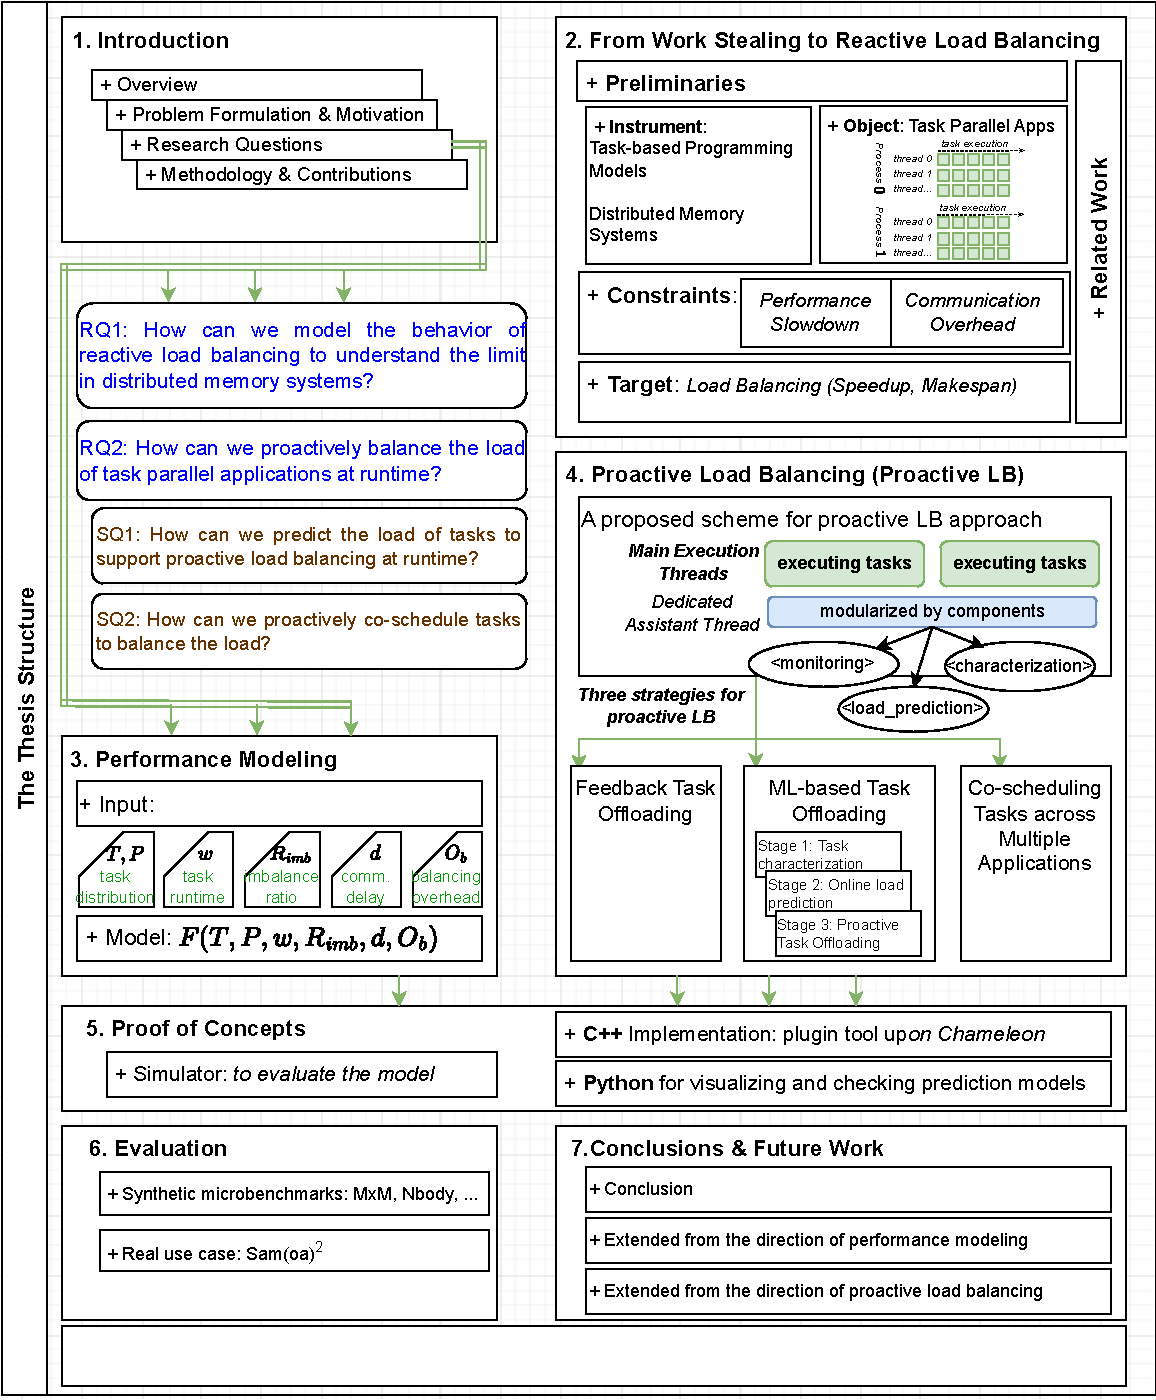
\includegraphics[scale=0.8]{./pictures/introduction/intro_thesis_outline.pdf}
	\caption{The structure of this thesis.}
	\label{fig:intro_outline}
\end{figure}

The structure of this thesis is shown in Figure \ref{fig:intro_outline}. The presented order emphasizes seven parts, where each indicates one chapter. Chapter \ref{ch:Introduction} highlights the overview of our topic and the problem formulation, leading to the motivation and research questions. Additionally, it also introduces the methodology and contribution. Chapter \ref{ch:wstoreactlb} is followed by From Work Stealing to Reactive Load Balancing. We aim to clarify the preliminaries, terminologies, and go through:
\begin{enumerate}
	\item Parallel Programming Models: implies the instruments we use to study dynamic load balancing.
	\item Task-based Parallel Applications: alludes to the object we use to study dynamic load balancing.
	\item Related Work: shows the taxonomy of dynamic load balancing and the state-of-the-art approaches in distributed memory systems. %The evaluation metrics are balancing ratio and speedup in completion time.
\end{enumerate}

Chapter \ref{ch:perfmodel} shows our performance model to analyze the bound of reactive load balancing approaches. The inputs are generalized as a given distribution of $T$ tasks on $P$ processes, the load value of tasks ($w$), imbalance ratio ($R_{imb}$), the overhead of task migration (delay time denoted by $d$) and balancing operation (denoted by $O_{\text{balancing}}$). The model focuses on possibilities when the existing approaches are bounded under the constraints of imbalance level and overhead. \\

Chapter \ref{ch:PADLB} introduces our new proactive load balancing approach. The main idea revolves around how we can predict the tasks' load values at runtime and better guide balancing by proactive task offloading. When we have more knowledge about load values, we can better estimate the number of tasks and potential processes. This approach facilitates two proactive task offloading methods: feedback task offloading and ML-based task offloading. Building upon proactive task offloading, we further introduce an extension of co-scheduling tasks across multiple applications. Our implementation offers a proactive scheme exploiting task-based programming models, where the main threads (execution threads) execute tasks, a dedicated thread ($Tcomm$) performs load prediction and proactive task offloading. For load prediction, $Tcomm$ performs characterizing tasks, training prediction models, and offloading tasks.\\
% Our approach is generally toward one approach which leverages different task offloading methods.

For evaluation, both simulator and reference implementation are used as proof of concepts in Chapter \ref{ch:PoC}. We describe the experiments in Chapter \ref{ch:Evaluation}, where we use synthetic microbenchmarks and a realistic use case of adaptive mesh refinement. Finally, we summarize the conclusions, discuss identified problems, and provide an outlook for future work in Chapter \ref{ch:ConclusionFutureWork}.\\




